\chapter{非惯性系；地球上的动力学}\label{ch:b1:non-inertial-frames}

站在向左转弯的公交车里，你会向右倾，
仿佛被一个无人施加的力推着。一桶放在转盘上旋转的水，
水面会凹陷成碗状。博物馆穹顶下的一个摆锤摆动了数小时，
摆动的平面每小时缓慢转过几度，
仿佛有一只看不见的手在转动它。这些都不是新的力：
它们正是描述运动的\omterm{def:b1:point-kinematics:frame}{参考系}本身在加速或转动时，牛顿定律呈现的样子。
本章说明速度与加速度如何在不同\omterm{def:b1:point-kinematics:frame}{参考系}之间变换，以及
动力学定律如何修正，
即通过加入\emph{\omterm{thm:b1:non-inertial-frames:dynamics}{惯性力}}，以及这些力
在最重要的转动\omterm{def:b1:point-kinematics:frame}{参考系}——地球上的作用。

\begin{omfigure}
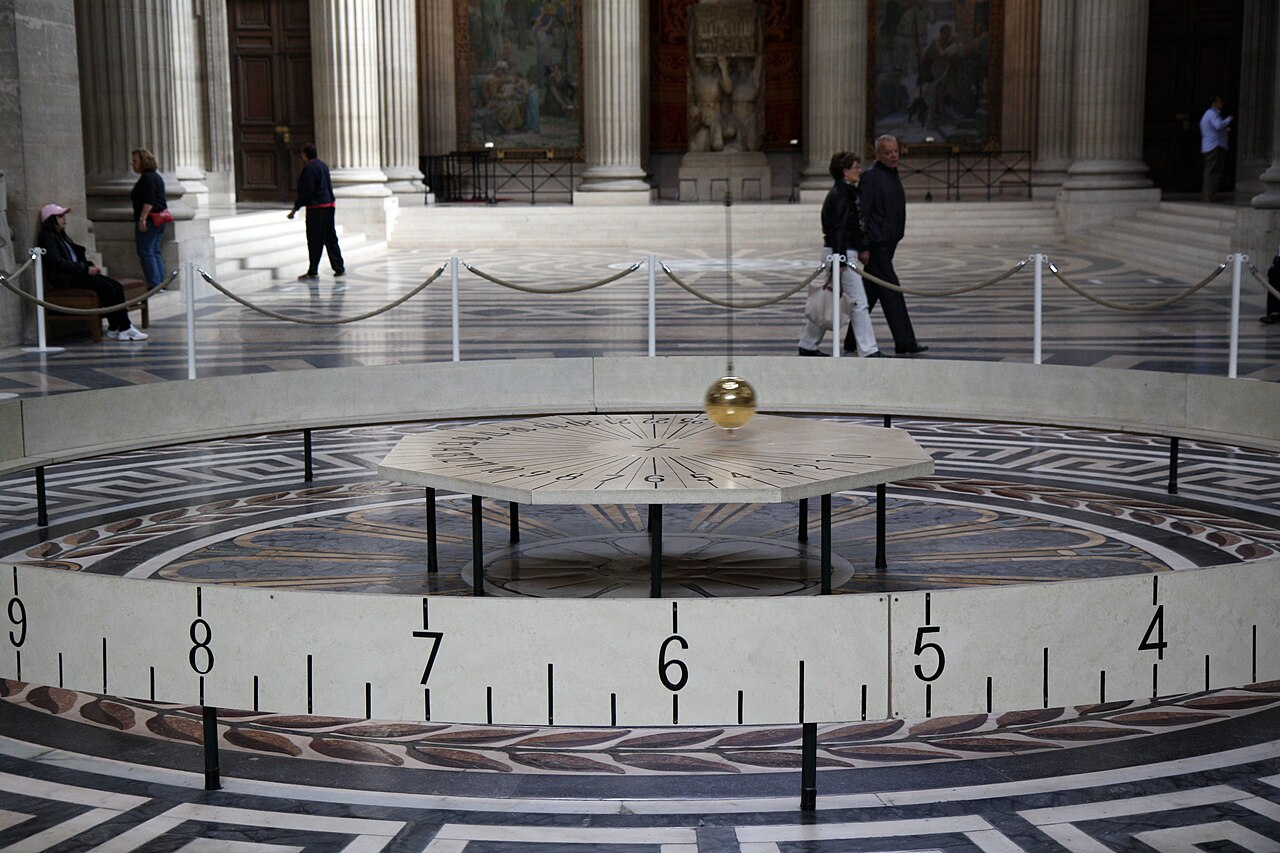
\includegraphics[width=0.55\linewidth]{images/book3/foucault-pendulum-pantheon.jpg}

{\small 巴黎先贤祠中的\omterm{prop:b1:non-inertial-frames:foucault}{傅科摆}，1851 年首次悬挂：钢丝长 \qty{67}{m}，摆锤质量 \qty{28}{kg}，摆动平面相对于地面转动。照片：Olga Khomitsevich，CC~BY~2.0。}
\end{omfigure}

\section{参考系的变换：运动学}

\begin{definition}[相对运动；平动参考系，定轴转动参考系]\label{def:b1:non-inertial-frames:frames}
\index{相对运动}\index{平动参考系}\index{定轴转动参考系}
设 $\mathcal R$ 为一\omterm{def:b1:point-kinematics:frame}{参考系}（原点为 $O$），$\mathcal R'$ 为与之相对运动的另一\omterm{def:b1:point-kinematics:frame}{参考系}（原点为
$O'$）。若 $\mathcal R'$ 的坐标轴
在 $\mathcal R$ 中的方向保持不变（$\mathcal R'$ 中每一点的速度都等于
$O'$ 的速度），则称之为\emph{平动}\omterm{def:b1:point-kinematics:frame}{参考系}。若 $\Delta$ 在两个\omterm{def:b1:point-kinematics:frame}{参考系}中都固定，
$\Delta$ 为转轴，$\mathcal R'$ 绕它
以\omterm{cor:b1:point-kinematics:circular}{角速度} $\Omega(t)$ 转动，则称之为\emph{定轴转动}\omterm{def:b1:point-kinematics:frame}{参考系}。
点 $M$ \emph{相对于} $\mathcal R'$ 的速度 $\vect v'$ 与加速度 $\vect a'$，
即 $\mathcal R'$ 中静止的观测者所测得的量。
\end{definition}

\begin{theorem}[速度与加速度的合成]\label{thm:b1:non-inertial-frames:composition}
\index{牵连速度}\index{牵连加速度}\index{科里奥利加速度}
\begin{itemize}
  \item $\mathcal R'$ 作平动，其速度为 $\vect v_{O'}$，
        加速度为 $\vect a_{O'}$：
        \[
        \vect v = \vect v' + \vect v_{O'}, \qquad \vect a = \vect a' + \vect a_{O'} .
        \]
  \item $\mathcal R'$ 绕固定轴 $\Delta$ 以 $\Omega$ 转动（矢量
        $\vect\Omega = \Omega\vect e_z$ 沿转轴方向）；$H$ 为
        $M$ 在转轴上的投影：
        \[
        \vect v = \vect v' + \vect\Omega\wedge\vect{HM}, \qquad
        \vect a = \vect a' + \underbrace{\big(-\Omega^2\vect{HM} + \dot\Omega\,\vect e_z\wedge\vect{HM}\big)}_{\vect a_e}
        + \underbrace{2\vect\Omega\wedge\vect v'}_{\vect a_C} .
        \]
\end{itemize}
$\vect a_e$ 为\emph{\omterm{thm:b1:non-inertial-frames:composition}{牵连加速度}}（即
$\mathcal R'$ 中与 $M$ 重合的点的加速度，
匀速转动时指向转轴的\omterm{cor:b1:point-kinematics:circular}{向心加速度}）；$\vect a_C = 2\vect\Omega\wedge\vect v'$ 为
\emph{\omterm{thm:b1:non-inertial-frames:composition}{科里奥利加速度}}，仅当 $M$ 相对于
转动\omterm{def:b1:point-kinematics:frame}{参考系}运动时才存在。
\end{theorem}

\begin{proof}
平动情形：$\vect{OM} = \vect{OO'} + \vect{O'M}$，其中
$\vect{O'M}$ 的分量取在共同基底中；对时间求两次导数。转动情形：
取绕 $\Delta$ 的\omterm{def:b1:point-kinematics:cylindrical}{柱坐标}，在 $\mathcal R$ 中为 $(r, \theta, z)$，
在 $\mathcal R'$ 中为 $(r, \theta', z)$，且 $\theta = \theta' + \int\Omega\,\dd t$。
于是由\cref{thm:b1:point-kinematics:cylindrical}，在 $\mathcal R$ 中取
$\dot\theta = \dot\theta' + \Omega$：
$\vect v = \dot r\vect e_r + r(\dot\theta' + \Omega)\vect e_\theta + \dot z\vect e_z
= \vect v' + r\Omega\vect e_\theta$，且 $r\Omega\vect e_\theta = \vect\Omega\wedge\vect{HM}$。
对加速度，取 $\ddot\theta = \ddot\theta' + \dot\Omega$：
$\vect a = [\ddot r - r(\dot\theta' + \Omega)^2]\vect e_r + [r(\ddot\theta' + \dot\Omega)
+ 2\dot r(\dot\theta' + \Omega)]\vect e_\theta + \ddot z\vect e_z$；展开并
合并同类项，得 $\vect a = \vect a' - r\Omega^2\vect e_r + r\dot\Omega\vect e_\theta
+ 2\Omega(-r\dot\theta'\vect e_r + \dot r\vect e_\theta)$，最后一个括号即为
$2\vect\Omega\wedge\vect v'$，由于 $\vect e_z\wedge\vect e_r = \vect e_\theta$，
$\vect e_z\wedge\vect e_\theta = -\vect e_r$。
\end{proof}

\begin{example}[在转盘上行走]\label{ex:b1:non-inertial-frames:turntable}
\cref{exo:b1:point-kinematics:12} 计算了一人沿径向以速率 $u$
在以 $\Omega$ 转动的转盘上行走时的加速度：$-ut\Omega^2\vect e_r
+ 2u\Omega\vect e_\theta$。用新的语言来说：相对加速度为零，
\omterm{thm:b1:non-inertial-frames:composition}{牵连加速度}为 $-r\Omega^2\vect e_r$，\omterm{thm:b1:non-inertial-frames:composition}{科里奥利加速度}为 $2\vect\Omega\wedge u\vect e_r = 2u\Omega\vect e_\theta$。
\end{example}

\section{非惯性系中的动力学：惯性力}

\begin{theorem}[非惯性系中的牛顿定律]\label{thm:b1:non-inertial-frames:dynamics}
\index{惯性力}\index{离心力}\index{科里奥利力}
在非惯性系 $\mathcal R'$ 中，质点的运动
满足
\[
m\vect a' = \sum\vect F + \vect F_e + \vect F_C, \qquad
\vect F_e = -m\vect a_e, \qquad \vect F_C = -m\vect a_C = -2m\vect\Omega\wedge\vect v' :
\]
牛顿第二定律即成立，只要在真实力之外再加上
\emph{牵连力}（对匀速转动的\omterm{def:b1:point-kinematics:frame}{参考系}，即
\emph{\omterm{thm:b1:non-inertial-frames:dynamics}{离心力}} $+m\Omega^2\vect{HM}$，方向背离转轴；
对\omterm{def:b1:non-inertial-frames:frames}{平动参考系}为 $-m\vect a_{O'}$），以及\emph{\omterm{thm:b1:non-inertial-frames:dynamics}{科里奥利
力}}。这些\emph{\omterm{thm:b1:non-inertial-frames:dynamics}{惯性力}}不是相互作用：没有任何物体施加它们，
它们也没有反作用力，并且
在惯性系中全部为零。
\end{theorem}

\begin{proof}
$m\vect a = \sum\vect F$ 在惯性系 $\mathcal R$ 中成立；代入
$\vect a = \vect a' + \vect a_e + \vect a_C$，并将两项移到
右边即可。
\end{proof}

\begin{example}[乘车的乘客与铅锤]\label{ex:b1:non-inertial-frames:bus}
在以 $a = \qty{3.0}{m/s^2}$ 减速行驶的公交车中，悬挂的吊环在
车内\omterm{def:b1:point-kinematics:frame}{参考系}中受到重力以及一个向前的\omterm{thm:b1:non-inertial-frames:dynamics}{惯性力} $ma$，它
沿\emph{视重力} $\vect g' = \vect g - \vect a_{O'}$ 的方向悬挂，
并向前倾斜 $\arctan(a/g) = 17^\circ$。想要站稳的乘客
必须向前倾，使身体对准这一视竖直方向。在自由
下落的电梯中，$\vect g' = \vect 0$：从内部看即为失重。
\end{example}

\begin{omfigure}
\begin{tikzpicture}[font=\small, x=1cm, y=1cm]
  % bus frame accelerating to the right (a): plumb bob tilts backward? braking: a points backward (left), bob tilts forward (right)
  \draw[thick] (-2.6,2.2) -- (2.6,2.2); \fill[pattern=north east lines] (-2.6,2.2) rectangle (2.6,2.4);
  \fill (0,2.2) circle (1.2pt);
  \draw[dashed] (0,2.2) -- (0,-0.2);
  \coordinate (B) at ($(0,2.2)+(-73:2.2)$);
  \draw[thick] (0,2.2) -- (B); \fill[omDef] (B) circle (3pt);
  \draw[-Stealth, omThm, very thick] (B) -- ++(0,-1.2) node[below] {$m\vect g$};
  \draw[-Stealth, omProp, very thick] (B) -- ++(0.9,0) node[right] {$-m\vect a_{O'}$};
  \draw[-Stealth, omExo, very thick] (B) -- ++(107:1.6) node[pos=0.6, left, xshift=-2pt] {$\vect T$};
  \draw (0,1.4) arc (-90:-73:0.8); \node at (0.3,1.15) {$\alpha$};
  \draw[-Stealth, thick] (-0.2,3.0) -- (-1.6,3.0); \node[below, font=\footnotesize] at (-0.9,2.95) {$\vect a_{O'}$（刹车）};
  \draw[-Stealth, thick] (0.4,3.0) -- (1.8,3.0); \node[below, font=\footnotesize] at (1.1,2.95) {运动};
  \begin{scope}[xshift=7.4cm]
  \draw[-Stealth, thick] (0,-0.4) -- (0,3.2) node[above] {$\Delta$};
  \draw[omDef!40, dashed] (0,1.0) ellipse (2.2 and 0.5);
  \fill[omDef] (2.2,1.0) circle (2.5pt) node[below right] {$M$};
  \draw[-Stealth, omProp, very thick] (2.2,1.0) -- ++(1.3,0) node[right] {$m\Omega^2\vect{HM}$};
  \draw[-Stealth, omExo, very thick] (2.2,1.0) -- ++(0.3,-0.95) node[below] {$-2m\vect\Omega\wedge\vect v'$};
  \draw[-Stealth, omThm, thick] (2.2,1.0) -- ++(-0.6,0.75) node[above] {$\vect v'$};
  \draw[-Stealth, omDef] (0.6,2.9) arc (80:20:0.6) node[right] {$\Omega$};
  \end{scope}
\end{tikzpicture}

{\small \omterm{thm:b1:non-inertial-frames:dynamics}{惯性力}。左：在刹车的公交车中，铅锤
沿表观重力 $\vect g - \vect a_{O'}$ 悬挂，向前倾斜。右图：
在以 $\Omega$ 旋转的\omterm{def:b1:point-kinematics:frame}{参考系}中，质点受到背离转轴的\omterm{thm:b1:non-inertial-frames:dynamics}{离心力}，
若质点运动，还受到与其
相对速度垂直的\omterm{thm:b1:non-inertial-frames:dynamics}{科里奥利力}。}
\end{omfigure}

\begin{example}[旋转的水桶]\label{ex:b1:non-inertial-frames:bucket}
绕竖直轴以 $\Omega$ 旋转的水桶中的水，
在重力与\omterm{thm:b1:non-inertial-frames:dynamics}{离心力}作用下相对旋转\omterm{def:b1:point-kinematics:frame}{参考系}静止：其自由面
与表观重力 $\vect g' = -g\vect e_z +
\Omega^2r\vect e_r$ 垂直（静止流体的自由面与场垂直，见
\cref{ch:b1:fluid-statics}）。其斜率为 $\dd z/\dd r = \Omega^2r/g$，于是
$z = \Omega^2r^2/2g$：抛物面。当 \qty{10}{rad/s} 时，
直径为 \qty{10}{cm} 的水桶，边缘比中心高出 \qty{5}{cm}——这正是
液态镜面望远镜的原理，其中旋转的汞
恰好呈现镜面所需的抛物形状。
\end{example}

\begin{method}[在非惯性参考系中求解]\label{met:b1:non-inertial-frames:method}
选取使问题最简单的\omterm{def:b1:point-kinematics:frame}{参考系}（公交车、转盘、
地球等）；列出真实力，加上 $-m\vect a_e$，若物体在该系中运动，
则再加上 $-2m\vect\Omega\wedge\vect v'$；然后按
\cref{met:b1:newton-dynamics:method}继续求解。检查：\omterm{thm:b1:non-inertial-frames:dynamics}{惯性力}绝不会
在能量平衡中表现为“某人所做的功”——\omterm{thm:b1:non-inertial-frames:dynamics}{科里奥利力}
与 $\vect v'$ 垂直，不做功；\omterm{thm:b1:non-inertial-frames:dynamics}{离心力}由\omterm{def:b1:work-and-energy:conservative}{势能}
$-\tfrac12 m\Omega^2r^2$ 导出，该\omterm{def:b1:work-and-energy:conservative}{势能}适用于
匀速旋转的\omterm{def:b1:point-kinematics:frame}{参考系}。
\end{method}

\section{地球参考系}

\begin{definition}[地心参考系与地球参考系]\label{def:b1:non-inertial-frames:earth}
\index{地心参考系}\index{地球参考系}
\emph{地心\omterm{def:b1:point-kinematics:frame}{参考系}}的原点位于地球中心，坐标轴指向
恒星；对于持续一天或更短时间的运动，它以极好的近似为
\omterm{thm:b1:newton-dynamics:laws}{惯性参考系}（其绕太阳运动的加速度
仅为 \qty{6e-3}{m/s^2}，在整个地球范围内近似均匀）。
\emph{地球\omterm{def:b1:point-kinematics:frame}{参考系}}固连于地面，相对于地心\omterm{def:b1:point-kinematics:frame}{参考系}
绕极轴以如下\omterm{cor:b1:point-kinematics:circular}{角速度}转动：
\[
\Omega = \frac{2\pi}{\qty{86164}{s}} = \qty{7.29e-5}{rad/s} .
\]
\end{definition}

\begin{proposition}[重力，以及 $g$ 的变化]\label{prop:b1:non-inertial-frames:weight}
\index{重力!与地球自转}
在\omterm{def:b1:non-inertial-frames:earth}{地球参考系}中，静止物体受到引力
$m\vect{\mathcal G}$ 与\omterm{thm:b1:non-inertial-frames:dynamics}{离心力} $m\Omega^2\vect{HM}$；二者的
合力即天平所测、铅垂线所示的量，亦即\emph{重力}
$m\vect g = m\vect{\mathcal G} + m\Omega^2\vect{HM}$。离心项在赤道处最大，
$\Omega^2R = \qty{0.034}{m/s^2}$，即 $0.35\%$ 的 $g$；它使 $g$ 自两极至赤道减小，
并使铅垂线偏离地心方向，
在中纬度处最大可达 $0.1^\circ$。
\end{proposition}

\begin{proof}
应用\cref{thm:b1:non-inertial-frames:dynamics}，取 $\vect v' = \vect 0$
（无\omterm{thm:b1:non-inertial-frames:dynamics}{科里奥利力}）；$\Omega^2R = (7.29\times10^{-5})^2 \times 6.37\times10^6$。
偏离角由 $m\vect{\mathcal G}$ 与\omterm{thm:b1:non-inertial-frames:dynamics}{离心力}所构成的三角形
得出（见\cref{exo:b1:non-inertial-frames:6}）。
\end{proof}

\begin{proposition}[地球上的科里奥利力]\label{prop:b1:non-inertial-frames:coriolis}
在纬度 $\lambda$ 处，以速率 $v'$ 水平运动的物体受到
大小为如下的水平\omterm{thm:b1:non-inertial-frames:dynamics}{科里奥利力}：
\[
F_C = 2m\Omega v'\sin\lambda ,
\]
其方向在北半球指向运动方向的\emph{右侧}，
在南半球则指向左侧，与前进方向无关；
竖直下落的物体则会被\emph{向东}偏转 $2m\Omega v'\cos\lambda$。
\end{proposition}

\begin{proof}
将 $\vect\Omega = \Omega(\cos\lambda\,\vect e_N + \sin\lambda\,\vect e_z)$ 分解为
（北向与当地竖直方向）。对于水平的 $\vect v'$，$-2m\vect\Omega\wedge\vect v'$
的水平分量为 $-2m\Omega\sin\lambda\,\vect e_z\wedge\vect v'$——
即从上方俯视，沿顺时针方向偏转 $90^\circ$ 而得的方向（相对于 $\vect v'$），当 $\lambda > 0$ 时——
以及竖直分量（与重力相比可以忽略）。对于竖直的 $\vect v' =
-v'\vect e_z$：$-2m\Omega\cos\lambda\,\vect e_N\wedge(-v'\vect e_z) = 2m\Omega v'\cos\lambda\,
\vect e_E$，向东。
\end{proof}

\begin{omfigure}
\begin{tikzpicture}[font=\small, x=1cm, y=1cm]
  \draw[omDef, thick] (0,0) circle (2.4);
  \draw[-Stealth, thick] (0,-3.0) -- (0,3.3) node[right] {$\vect\Omega$};
  \draw[dashed] (-2.6,0) -- (2.6,0);
  \coordinate (P) at (45:2.4);
  \fill[omThm] (P) circle (2pt);
  \draw[-Stealth, omThm, thick] (P) -- ++(45:1.0) node[right] {$\vect e_z$};
  \draw[-Stealth, omThm, thick] (P) -- ++(135:1.0) node[above left] {$\vect e_N$};
  \draw (0.9,0) arc (0:45:0.9); \node at (0.7,0.35) {$\lambda$};
  \draw[-Stealth, omExo, thick] (P) -- ++(45:0.45) ++(0,0) -- ++(0,0);
  \draw[-Stealth, omProp, very thick] (P) -- ++(0,1.2) node[above right] {$\vect\Omega$（当地）};
  \node[omProp, font=\footnotesize] at (3.0,1.2) {$\Omega\sin\lambda\,\vect e_z + \Omega\cos\lambda\,\vect e_N$};
  \begin{scope}[xshift=7.8cm]
  \draw[-Stealth] (-1.8,0) -- (2.0,0) node[right] {东};
  \draw[-Stealth] (0,-1.6) -- (0,2.0) node[above] {北};
  \draw[-Stealth, omThm, very thick] (0,0) -- (0,1.4) node[left] {$\vect v'$};
  \draw[-Stealth, omExo, very thick] (0,0.7) -- (1.1,0.7) node[right] {$\vect F_C$};
  \draw[omDef, thick, domain=0:1.5, samples=40] plot ({0.35*\x*\x},{\x});
  \node[font=\footnotesize] at (0.8,-0.9) {从上方俯视，$\lambda > 0$};
  \end{scope}
\end{tikzpicture}

{\small 左：在纬度 $\lambda$ 处，地球自转矢量具有
竖直分量 $\Omega\sin\lambda$ 与北向分量 $\Omega\cos\lambda$。
右：从北半球上方俯视，沿水平方向运动的物体
受\omterm{thm:b1:non-inertial-frames:dynamics}{科里奥利力}推向其右侧，其\omterm{def:b1:point-kinematics:frame}{轨迹}
顺时针弯曲。}
\end{omfigure}

\begin{example}[微小的力，巨大的后果]\label{ex:b1:non-inertial-frames:coriolisnum}
位于纬度 $45^\circ$ 处、以 \qty{100}{km/h} 行驶的火车：$a_C = 2 \times 7.29\times
10^{-5} \times 27.8 \times 0.71 = \qty{2.9e-3}{m/s^2}$，
即 $g$ 的千分之三——单向行驶的铁轨中，右侧钢轨磨损略快。
空气以 \qty{20}{m/s} 流向低压中心，
一路向右偏转，最终绕中心逆时针旋转：
北半球的每个气旋都这样转，南半球的则相反。一块石子
在纬度 $45^\circ$ 处自 \qty{100}{m} 深的竖井落下，
落点位于铅垂线以东 \qty{1.6}{cm} 处（见\cref{exo:b1:non-inertial-frames:7}）。
\end{example}

\begin{proposition}[傅科摆]\label{prop:b1:non-inertial-frames:foucault}
\index{傅科摆}
在纬度 $\lambda$ 处以小\omterm{def:b1:wave-propagation:signal}{振幅}摆动的\omterm{ex:b1:newton-dynamics:pendulum}{单摆}，
其摆动平面相对于\omterm{def:b1:non-inertial-frames:earth}{地心参考系}的当地竖直轴保持不变，
仅相对于地球本身而言会转动。在\omterm{def:b1:non-inertial-frames:earth}{地球参考系}中看，摆动平面以
\emph{顺时针}方向转动（从北半球上方看），角速率为
$\Omega\sin\lambda$，即转过一周所需的时间为
\[
T_F = \frac{\qty{23.93}{h}}{\sin\lambda} .
\]
\end{proposition}

\begin{proof}[部分证明]
在极点（$\lambda = 90^\circ$）处，论证是几何性的：
除张力外，摆锤不受水平方向的力，张力的水平分量
沿摆动方向，因此在\omterm{def:b1:non-inertial-frames:earth}{地心参考系}中摆动平面保持固定，
而地球在其下以 $\Omega$ 转动；从地面看，摆动平面以 $-\Omega$ 转动。
在纬度 $\lambda$ 处，水平方向的\omterm{thm:b1:non-inertial-frames:dynamics}{科里奥利力}为
$-2m\Omega\sin\lambda\,\vect e_z\wedge\vect v'$，恰是绕当地竖直方向以
$\Omega\sin\lambda$ 转动的\omterm{def:b1:point-kinematics:frame}{参考系}所产生的力。在
随摆动平面以 $-\Omega\sin\lambda$ 转动的\omterm{def:b1:point-kinematics:frame}{参考系}中，该力在一阶近似下消失，
摆即为普通的平面振子，因此摆动平面
在\omterm{def:b1:non-inertial-frames:earth}{地球参考系}中以 $\Omega\sin\lambda$ 进动。完整的计算，
连同被略去的二阶项，是
周末问题。
\end{proof}

\begin{remark}[两句话说清潮汐]\label{rem:b1:non-inertial-frames:tides}
\index{潮汐}
在随地心自由下落、朝向月球运动的\omterm{def:b1:point-kinematics:frame}{参考系}中，
月球的引力并不均匀：近月一侧稍强，
远月一侧稍弱。二者之差的量级为 $2GM_{\text{月球}}R/d^3
\approx \qty{1e-6}{m/s^2}$，使海洋拉伸成两个隆起——一天两次
\omterm{rem:b1:non-inertial-frames:tides}{潮汐}——太阳的贡献为月球的 $46\%$，
使大潮与小潮随二者对齐或交叉而形成
（见\cref{exo:b1:non-inertial-frames:12}）。
\end{remark}

\section{练习}

\begin{exercise}[$\star$]\label{exo:b1:non-inertial-frames:1}
一铅锤悬挂于以 \qty{2.5}{m/s^2} 加速行驶的汽车中，求其与竖直方向的夹角，
以及以 $mg$ 为单位的张力。若同一汽车以
相同加速度制动，结果如何？
\end{exercise}

\begin{exercise}[$\star$]\label{exo:b1:non-inertial-frames:2}
一个孩子坐在距旋转木马转轴 \qty{3.0}{m} 处，木马每
\qty{4.0}{s} 转一周。求旋转\omterm{def:b1:point-kinematics:frame}{参考系}中的离心加速度，用 $g$ 的
分数表示；是什么真实的力提供了这一加速度？
\end{exercise}

\begin{exercise}[$\star$]\label{exo:b1:non-inertial-frames:3}
求地球的\omterm{cor:b1:point-kinematics:circular}{角速度} $\Omega$、赤道处的离心加速度
及其占 $g$ 的比例。在何种自转周期下，赤道上的
物体会脱离地面？
\end{exercise}

\begin{exercise}[$\star$]\label{exo:b1:non-inertial-frames:4}
一列质量为 \qty{400}{t} 的火车，在纬度 $45^\circ$ 处以 \qty{100}{km/h} 行驶。
求\omterm{thm:b1:non-inertial-frames:composition}{科里奥利加速度}及钢轨受到的侧向力；
哪一根钢轨受到推挤？向北与向东行驶时各如何？
\end{exercise}

\begin{exercise}[$\star\star$]\label{exo:b1:non-inertial-frames:5}
一个半径为 \qty{10}{cm} 的水桶先以 \qty{2.0}{rad/s} 转动，
再以 \qty{10}{rad/s} 转动。求边缘处水面相对中心的升高。
为什么旋转的水银槽可以作为望远镜的好镜子？
\end{exercise}

\begin{exercise}[$\star\star$]\label{exo:b1:non-inertial-frames:6}
证明：纬度 $\lambda$ 处的铅垂线偏离地心的角度
约为 $\Omega^2R\sin\lambda\cos\lambda/g$ 弧度，并计算
在 $45^\circ$ 处以角分为单位表示。仅由自转引起，赤道处的 $g$ 比
极点处小多少？
\end{exercise}

\begin{exercise}[$\star\star$]\label{exo:b1:non-inertial-frames:7}
一块石子在纬度 $45^\circ$ 处从静止开始落入 \qty{100}{m} 深的竖井。
将\omterm{thm:b1:non-inertial-frames:composition}{科里奥利加速度} $2\Omega v\cos\lambda$（向东）视为小量，
取 $v = gt$，两次积分求出
底部的向东偏离量。为什么偏向东方？
\end{exercise}

\begin{exercise}[$\star\star$]\label{exo:b1:non-inertial-frames:8}
求巴黎（$\lambda = 48.9^\circ$）处\omterm{prop:b1:non-inertial-frames:foucault}{傅科摆}的进动周期，
以及极点处与赤道处的进动周期。摆动平面在
巴黎一小时内转过多大角度？
\end{exercise}

\begin{exercise}[$\star\star$]\label{exo:b1:non-inertial-frames:9}
空气以 \qty{20}{m/s} 流向位于 $45^\circ$
北纬处的低压中心。求\omterm{thm:b1:non-inertial-frames:composition}{科里奥利加速度}，并判断空气最终
绕中心旋转的方向。为什么小尺度的涡旋（如下水口的漩涡、龙卷风）不遵循
这一规律？
\end{exercise}

\begin{exercise}[$\star\star\star$]\label{exo:b1:non-inertial-frames:10}
一个系着绳子的氦气球漂浮在汽车内。当汽车
向前加速时，气球会向哪个方向倾斜？请用
视重力和浮力加以解释。
\end{exercise}

\begin{exercise}[$\star\star\star$]\label{exo:b1:non-inertial-frames:11}
空间站是一个半径为 \qty{100}{m} 的圆环，通过自转使其边缘处产生 $1g$ 的
人工重力。求旋转周期。一名宇航员沿边缘行走，
速度为 \qty{1.5}{m/s}：求\omterm{thm:b1:non-inertial-frames:composition}{科里奥利加速度}，以及他顺着与逆着旋转方向行走时
其视重所受的影响。他从 \qty{2.0}{m} 高处释放一个小球，
求小球落地点距其脚下的大致距离。
\end{exercise}

\begin{exercise}[$\star\star\star$]\label{exo:b1:non-inertial-frames:12}
证明：月球引力加速度在地心处与地表最靠近月球的点处
之差约为
$2GM_Mr/d^3$（其中 $r$ 为地球半径，$d$ 为地月距离）；
计算该差值，并对太阳作同样计算；由此推出
太阳\omterm{rem:b1:non-inertial-frames:tides}{潮汐}与月球\omterm{rem:b1:non-inertial-frames:tides}{潮汐}之比。
\end{exercise}

\section{问题：傅科摆}

\begin{problem}[{周末问题——穹顶下系于 67 米细线上的 28 千克摆锤：
摆动平面为何转动、转动多快、它证明了什么，
以及使其转动的力有多小}]
\label{pb:b1:non-inertial-frames:1}
1851 年，一个摆长为 $\ell = \qty{67}{m}$、质量为 $m = \qty{28}{kg}$ 的
摆在巴黎先贤祠的穹顶下摆动，纬度 $\lambda =
48.85^\circ$，\omterm{def:b1:wave-propagation:signal}{振幅}约为 $x_0 = \qty{3.0}{m}$。$\Omega =
\qty{7.29e-5}{rad/s}$，$g = \qty{9.81}{m/s^2}$。

\medskip
\noindent\textbf{第一部分——摆本身。}
\begin{enumerate}
  \item 求微\omterm{prop:b1:work-and-energy:stability}{小振动}的周期；检验\omterm{def:b1:wave-propagation:signal}{振幅}是否足够小（
        （$x_0/\ell$）。
  \item 求摆锤的最大速率，以及其
        离最低点的最大高度。
  \item 求最低点处的张力，以 $mg$ 为单位表示。
  \item 估算摆锤在最大速率时受到的空气阻力（
        平方律，$C_xS \approx \qty{0.05}{m^2}$，$\rho = \qty{1.2}{kg/m^3}$），并
        与最大回复力 $m\omega_0^2x_0$ 作比较。
  \item 为什么要用长线和重摆锤？（给出两个理由，一个与周期有关，
        另一个与阻尼有关。）
\end{enumerate}

\medskip
\noindent\textbf{第二部分——在极点处。}
设想同一个摆位于北极点。
\begin{enumerate}[resume]
  \item 在\omterm{def:b1:non-inertial-frames:earth}{地心参考系}中列出作用于摆锤上的力，
        并说明没有任何力能使其摆动平面发生转动。
  \item 推出站在冰面上的观察者看到摆动平面如何转动，
        以及经过多长时间它会回到初始方向。
  \item 描述摆锤在地面上的\omterm{def:b1:point-kinematics:frame}{轨迹}（玫瑰线）：一天内
        有多少个花瓣？
\end{enumerate}

\medskip
\noindent\textbf{第三部分——在纬度 $\lambda$ 处：科里奥利项。}
取局部坐标轴：$x$ 指向东，$y$ 指向北，$z$ 竖直向上；由于是微\omterm{prop:b1:work-and-energy:stability}{小振动}，
运动近似水平，$\vect v' \approx (\dot x, \dot y, 0)$；
回复力为 $-m\omega_0^2(x, y, 0)$，其中 $\omega_0 = \sqrt{g/\ell}$。
\begin{enumerate}[resume]
  \item 在这些坐标轴中写出 $\vect\Omega$。
  \item 计算 $-2m\vect\Omega\wedge\vect v'$，并保留其水平分量；
        证明它们只含 $\Omega\sin\lambda$。
  \item 写出 $x$ 与 $y$ 的两个运动方程；令
        $\omega_F = \Omega\sin\lambda$，并比较 $\omega_F$ 与 $\omega_0$。
  \item 引入 $u = x + jy$，证明 $\ddot u + 2j\omega_F\dot u +
        \omega_0^2u = 0$。
  \item 设 $u = \eu^{j\alpha t}$，求 $\alpha$ 的两个值，并
        证明当 $\omega_F \ll \omega_0$ 时，它们近似为 $\alpha \approx \pm\omega_0
        - \omega_F$。
  \item 推出 $u \approx \eu^{-j\omega_Ft}(A\eu^{j\omega_0t} + B\eu^{-j\omega_0t})$：
        解释因子 $\eu^{-j\omega_Ft}$——摆动平面以何种方式、
        以何种速率转动？
  \item 计算巴黎的进动周期，以及
        一小时内转过的角度。
  \item 为什么摆动平面在赤道处不发生转动？
\end{enumerate}

\medskip
\noindent\textbf{第四部分——这个力有多小。}
\begin{enumerate}[resume]
  \item 求作用于摆锤上的最大\omterm{thm:b1:non-inertial-frames:dynamics}{科里奥利力}，并将其
        与重力及最大回复力作比较。
  \item 在半个周期内，摆动端点在侧向上位移了多少？
        （摆动平面转过 $\omega_FT/2$。）
  \item 1851 年，摆锤上装有一支尖笔，它会碰倒
        在\omterm{def:b1:wave-propagation:signal}{振幅}处排成圆环的小钉子：下一颗钉子倒下前
        大约需要多长时间？
  \item 摆是通过烧断把摆锤拉向一侧的细线来释放的。
        为什么不直接用手推它？
  \item 空气阻力会在几小时后使摆停止。现代博物馆的
        摆在底部装有一个小电磁铁，用以补充能量，
        而不触及摆动平面：为什么这一冲量必须
        严格沿径向？
\end{enumerate}

\medskip
\noindent\textbf{第五部分——它证明了什么，以及还有什么作用。}
\begin{enumerate}[resume]
  \item 傅科的演示使公众确信了地球的
        自转。进动速率究竟测量的是什么？该实验
        能否确定纬度？
  \item 在哪个纬度，摆动平面恰好在 \qty{48}{h} 内转过一周？
  \item 陀螺仪（一个安装在万向支架中的高速旋转轮子）的轴
        在\omterm{def:b1:non-inertial-frames:earth}{地心参考系}中保持不变。用一句话解释它为何也能
        揭示地球的自转，并举出一个应用。
  \item 总结：起作用的唯一\omterm{thm:b1:non-inertial-frames:dynamics}{惯性力}、其对纬度的依赖关系，
        以及它在巴黎给出的周期。
\end{enumerate}
\end{problem}
